% ─────────────────────────────────────────────────────────────────────────────
\section{System Model}
% ─────────────────────────────────────────────────────────────────────────────

This section describes the mathematical and logical structure of the simulation. We define the environment and the behaviors of each agent type to provide a clear view of the swarm dynamics.

\paragraph{The Environment}
The simulation takes place in a continuous area of $45 \times 25$ meters, as shown in Figure~\ref{fig:simulation}. We overlay this space with a shared pheromone grid to coordinate the swarm. Colored squares on the map indicate recently visited locations, where the intensity of the coverage can be read from the legend on the right. This space is inhabited by two UAV agents and five Victim agents. The Victim agents act as passive data containers that store their specific location and discovery status. They contain no internal logic and remain stationary throughout the mission for the sake of simplicity. The Main agent then orchestrates the simulation by initializing the environment and placing targets according to a GMM. This orchestrator also manages the pheromone grid and applies a lazy exponential decay model to simulate evaporation over time:
\begin{equation}
    \tau(t) = \tau_0 \cdot e^{-\rho (t - t_0)} .
\end{equation}
In this model, $\tau(t)$ represents the current pheromone level, and $\tau_0$ is the level recorded at the last update time $t_0$. The parameter $\rho$ sets the evaporation rate. This decay ensures that the spatial memory of the swarm remains dynamic and responsive to recent sensor data.

% ─────────────── Full-width simulation figure ─────────────────────────────
\begin{figure*}[ht]
    \centering
    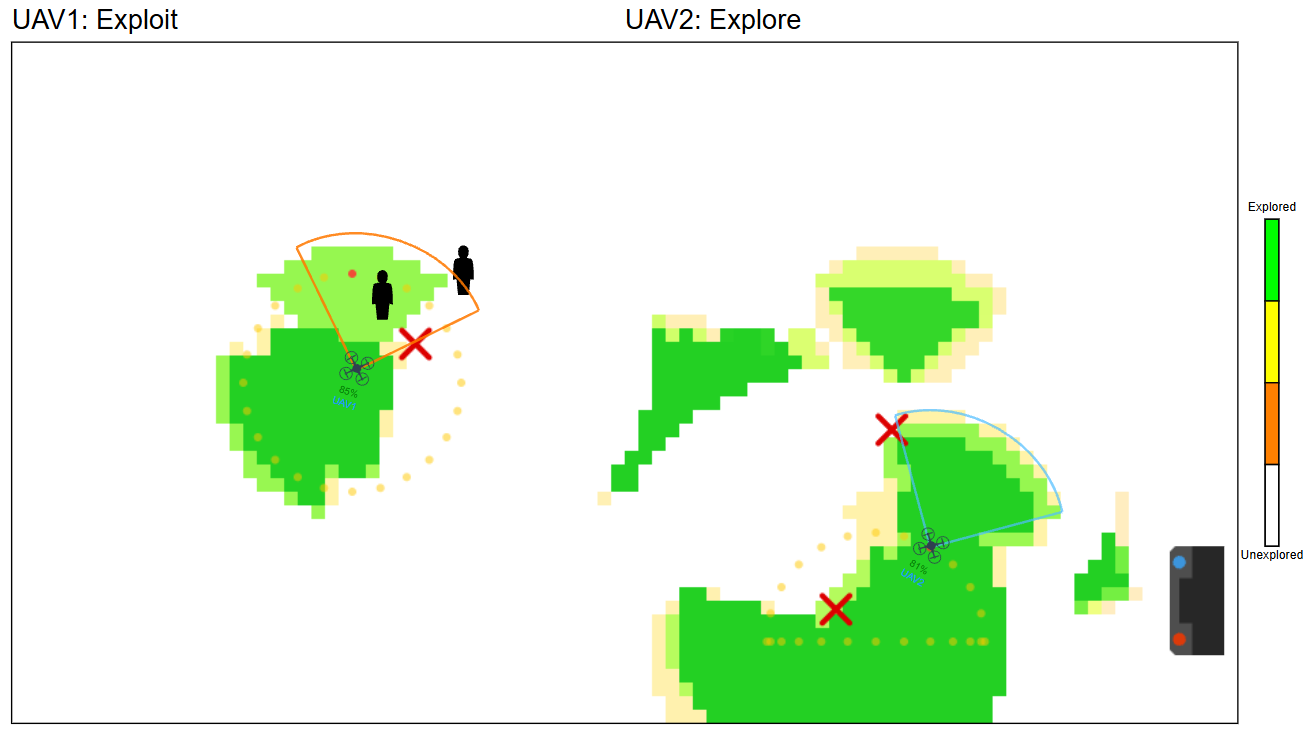
\includegraphics[width=\textwidth]{img/simulation.png}
    \caption{Snapshot of the running simulation showing the pheromone distribution, where green tones indicate high coverage and white indicates unexplored territory. UAV2 on the right is in \texttt{Explore} mode, with its blue sensor cone sweeping the area ahead. UAV1 on the left is in \texttt{Exploit} mode, with an orange cone indicating an active victim detection. Red crosses mark victims that have already been confirmed.}
    \label{fig:simulation}
\end{figure*}

\paragraph{Agent Behaviour}
Once the environment is set up, we define how the agents behave within it. Each UAV follows a BDI architecture implemented through the hierarchical state chart shown in Figure~\ref{fig:statechart}. At the start of the mission, agents enter a \texttt{Startup} phase to reach pre-assigned dispersal positions. This ensures that the fleet begins the search with minimal overlap. Once in position, each UAV enters the main behavioural cycle, where it switches between the \texttt{Explore} and \texttt{Exploit} parent states. An orthogonal state called \texttt{BatteryDischarge} runs in parallel throughout the flight to simulate the continuous depletion of the battery at a constant rate.

\paragraph{Searching for Victims}
The core of this behavioural cycle is the search process within the \texttt{Explore} parent state. This mode implements a reversed ACO logic to cover the area. As shown in Figure~\ref{fig:simulation}, each UAV considers a ring of $n$ yellow candidate waypoints. The radius of this ring is called the step length $d$. The agent scores each candidate $i$ based on the local pheromone level $\tau_i$ and the staleness $\eta_i$ of the grid cell:
\begin{equation}
    s_i = \left(\frac{1}{1 + \tau_i}\right)^{\alpha} \cdot \eta_i^{\beta} .
\end{equation}
In this scoring function, $\alpha$ and $\beta$ are exponents that weight the importance of pheromone repulsion and staleness attraction. Staleness is derived from the freshness $f_i$ of a cell, which tracks the time since it was last sensed:
\begin{equation}
    f_i(t) = \max\left(0,\; 1 - \frac{t - t_{\mathrm{last},i}}{T_{\mathrm{stale}}}\right) .
\end{equation}
The term $t_{\mathrm{last},i}$ is the timestamp of the last visit, and $T_{\mathrm{stale}}$ is a constant that defines when a cell is considered completely stale. Within the \texttt{ExploreSense} and \texttt{ExplorePlan} sub-states, the agent evaluates these scores and chooses a destination marked by a red circle in the simulation. The UAV then transitions to \texttt{ExploreMove} to fly toward the target.

If the local area is already heavily covered, an \texttt{ExploreAdaptStep} node allows the UAV to escape the saturated neighbourhood. This mechanism checks the minimum pheromone level $\tau_{\min}$ among all candidates on the ring. When $\tau_{\min}$ is high, it indicates that even the least-explored candidate is in a well-covered region. In this case, the UAV increases its step length to jump further into fresh territory:
\begin{equation}
    d_{\mathrm{current}} = d \cdot \min\left(M,\; 1 + \tau_{\min}\right) .
\end{equation}
The parameter $M$ acts as a maximum multiplier to keep the jump distance within a reasonable range. This adaptive behaviour prevents the UAV from wasting time in areas that have already been thoroughly searched.

\vspace{1cm}
\paragraph{Confirming detections}
A detection within the sensor cone initiates a transition to the \texttt{Exploit} parent state. As shown in Figure \ref{fig:simulation}, this shift is visible when the sensor cone of a UAV changes from blue to orange. The agent first enters the \texttt{ExploitVerify} sub-state to confirm the signal through a secondary sensing sweep before navigating to the target. Once the UAV reaches the victim, the \texttt{ExploitConfirm} state handles the final logging and mission statistics. This discovery is marked with a red cross on the map and the Main agent clears the nearby pheromone grid. The white unexplored zone surrounding the victim in the bottom right of Figure \ref{fig:simulation} illustrates this reset which encourages the swarm to re-examine the area. After the confirmation is complete, the agent returns to the \texttt{Explore} mode.

\paragraph{Battery and Charging}
When the battery level drops below a set threshold, the agent preempts its current task and enters the \texttt{ChargingStation} parent state. During the \texttt{MovingToCharger} phase, the UAV suspends non-essential operations like sensing and pheromone deposition. This energy saving mode halves the battery depletion rate while the agent travels toward the charging station at the bottom right of the environment. After reaching this location, the UAV enters the \texttt{Charging} sub-state to replenish its power. Once the battery is fully recharged, the agent uses its saved coordinates to return to the search area and resume its mission.
